\chapter{DAME M\'AS GASOLINA Y OTRAS FORMAS DE GASTO}\label{chap:fepc}

Como se mostró en el capítulo anterior, las dificultades fiscales que enfrenta Colombia actualmente tienen su origen, en gran medida, en la imposibilidad de retornar a la senda de gasto público que existía antes de la pandemia. No obstante, reducir ese gasto adicional enfrenta unos desafíos legales, económicos y políticos que se discuten en este capítulo.

Para entender estos desafíos, es necesario revisar los componentes del gasto publico. Después de todo, el ajuste por el lado del gasto implica decidir no solo \textit{cuánto} recortar, sino también \textit{qué} recortar. En la contabilidad fiscal, el gasto público se divide usualmente en tres grandes componentes: el pago de intereses sobre la deuda, la inversión pública y el gasto de funcionamiento. No obstante, esta desagregación lleva a pensar que, dado el alto peso del gasto de funcionamiento sobre el total de gasto, el gasto del Gobierno Nacional Central (\gls{gnc}) está constituido más que todo por burocracia. Nada más lejos de la realidad.

\input{Tablas/Cap02/GastoDesagregado}

La Tabla \ref{tab:GastoDesagregado} presenta la evolución del gasto público entre 2019 y 2024, utilizando una desagregación distinta a la tradicional clasificación entre funcionamiento, inversión e intereses. En su lugar, el gasto se divide en cinco categorías: intereses (pagos por obligaciones financieras derivadas de la deuda pública), inversión (destinada a proyectos de infraestructura y activos de largo plazo), gasto de personal (remuneraciones y contribuciones asociadas a los empleados públicos), adquisición de bienes y servicios (donde se incluyen los contratistas por prestación de servicios), y transferencias (recursos asignados a hogares, empresas, instituciones y gobiernos subnacionales). En todos los años considerados, las transferencias no solo representan la mayor proporción del gasto público, sino que superan la suma combinada de todos los demás componentes.

La misma tabla permite identificar que los principales responsables del aumento del gasto público en este período fueron los intereses y, en mayor medida, las transferencias. Entre 2019 y 2024, el pago de intereses se incrementó en 1,4 puntos del PIB. Por su parte, las transferencias aumentaron en 2,9 puntos del PIB, convirtiéndose en el principal factor del crecimiento del gasto. En conjunto, estos dos rubros explican casi la totalidad del aumento de 4,5 puntos del PIB en el gasto público observado durante el periodo.

\section{Transferencias}

El creciente peso de las transferencias dentro del gasto público, especialmente a partir de la pandemia, subraya la necesidad de examinar con mayor detalle la composición de estos rubros en cualquier discusión sobre ajuste fiscal. La Tabla \ref{tab:Transferencias} presenta una desagregación de las transferencias y su evolución reciente, ordenadas de mayor a menor según su valor en 2024. De la tabla se desprende que tres componentes explican la mayor parte del incremento del gasto primario entre 2019 y 2024: en primer lugar, el subsidio a los combustibles, reflejado en la transferencia para cerrar el déficit del Fondo para la Estabilización del Precio de los Combustibles (\gls{fepc}); en segundo lugar, las transferencias al sistema de salud; y en tercer lugar, las pensiones. No obstante, cerca de 0,5 puntos porcentuales del aumento total en transferencias durante este periodo no se pueden asociar a partidas específicas, pues corresponden a rubros no desagregados en la contabilidad fiscal disponible.

A continuación, se examina brevemente la evolución reciente de seis transferencias que en al menos algún momento entre 2019 y 2024 tuvieron un peso relativo importante: 1) el pago de pensiones, 2) las transferencias a las regiones a través del Sistema General de Participaciones (\gls{sgp}), 3) las transferencias al sistema de salud, 4) el subsidio a los combustibles, 5) el Fondo de Mitigación de Emergencias (\gls{fome}), y 6) el \gls{sena} y el \gls{icbf}.

\begin{table}[h!]
\centering
\caption{Desagregación de Transferencias del GNC (\% PIB)}
\label{tab:Transferencias}
\resizebox{\textwidth}{!}{%
\begin{tabular}{l|cccccc|c}
\hline
\textbf{Concepto} & \textbf{2019} & \textbf{2020} & \textbf{2021} & \textbf{2022} & \textbf{2023} & \textbf{2024} & \textit{\textbf{2024–2019}} \\ \hline
SGP & 3,9 & 4,3 & 3,9 & 3,3 & 3,3 & 4,0 & \textit{0,1} \\
Pensiones$^1$ & 3,2 & 4,3 & 3,6 & 2,9 & 3,6 & 3,6 & \textit{0,4} \\
Salud$^2$ & 1,7 & 1,9 & 2,1 & 1,9 & 2,2 & 2,4 & \textit{0,7} \\
FEPC & 0,0 & 0,0 & 0,0 & 1,2 & 1,7 & 1,2 & \textit{1,2} \\
SENA e ICBF$^3$ & 0,2 & 0,3 & 0,3 & 0,2 & 0,2 & 0,2 & \textit{0,0} \\
Universidades & 0,3 & 0,4 & 0,3 & 0,3 & 0,3 & 0,4 & \textit{0,1} \\
Subsidios Servicios Públicos & 0,2 & 0,3 & 0,3 & 0,2 & 0,3 & 0,2 & \textit{0,0} \\
Cesantías y Salud FOMAG & 0,1 & 0,1 & 0,2 & 0,1 & 0,1 & 0,1 & \textit{0,0} \\
Deudas Entidades & 0,1 & 0,1 & 0,1 & 0,1 & 0,3 & 0,1 & \textit{0,0} \\
Sentencias & 0,1 & 0,1 & 0,1 & 0,1 & 0,1 & 0,1 & \textit{0,0} \\
FOME y FNG & 0,0 & 1,9 & 2,0 & 0,2 & 0,0 & 0,0 & \textit{0,0} \\
Resto$^4$ & 0,7 & 0,9 & 1,4 & 0,9 & 1,0 & 1,2 & \textit{0,5} \\ \hline
\textbf{Total Transferencias*} & \textbf{10,6} & \textbf{14,5} & \textbf{14,2} & \textbf{11,4} & \textbf{13,2} & \textbf{13,5} & \textit{\textbf{2,9}} \\ \hline
\end{tabular}%
}
\vspace{0.1cm}
\par \footnotesize{$^1$ Incluye bonos pensionales.}
\par \footnotesize{$^2$ Incluye 4,4 de los 9 puntos del antiguo CREE.}
\par \footnotesize{$^3$ Corresponde a 3,6 de los 9 puntos del antiguo CREE.}
\par \footnotesize{$^4$ Incluye a 1 de los 9 puntos del antiguo CREE.}
\par \footnotesize{*Excluye reclasificaciones por contribuciones a la nómina.}
\vspace{0.1cm}
\par \footnotesize{\textit{Fuente: Elaboración propia con base en \textcite{minhacienda_balance_2025}.}}
\end{table}

\begin{comment}
\begin{table}[h!]
\centering
\caption{Desagregación de Transferencias del GNC (\% PIB)}
\label{tab:Transferencias}
\resizebox{\textwidth}{!}{%
\begin{tabular}{l|cccccc|c}
\hline
\textbf{Concepto} & \textbf{2019} & \textbf{2020} & \textbf{2021} & \textbf{2022} & \textbf{2023} & \textbf{2024} & \textit{\textbf{(2024–2019)}} \\ \hline
SGP & 3,9 & 4,3 & 3,9 & 3,3 & 3,3 & 4,0 & \textit{0,1} \\
Pensiones y bonos pensionales & 3,2 & 4,3 & 3,6 & 2,9 & 3,6 & 3,6 & \textit{0,4} \\
Aseguramiento en Salud & 1,4 & 1,6 & 1,8 & 1,7 & 1,9 & 2,1 & \textit{0,7} \\
FEPC & 0,0 & 0,0 & 0,0 & 1,2 & 1,7 & 1,2 & \textit{1,2} \\
SENA e ICBF & 0,6 & 0,7 & 0,6 & 0,5 & 0,5 & 0,6 & \textit{0,0} \\
Universidades & 0,3 & 0,4 & 0,3 & 0,3 & 0,3 & 0,4 & \textit{0,1} \\
FOME y FNG & 0,0 & 1,9 & 2,0 & 0,2 & 0,0 & 0,0 & \textit{0,0} \\
Resto & 1,2 & 1,3 & 2,0 & 1,4 & 1,7 & 1,7 & \textit{0,5} \\ \hline
\textbf{Total Transferencias*} & \textbf{10,6} & \textbf{14,5} & \textbf{14,2} & \textbf{11,4} & \textbf{13,2} & \textbf{13,5} & \textit{\textbf{2,9}} \\ \hline
\end{tabular}%
}
\vspace{0.1cm}
\par \footnotesize{*Excluye reclasificaciones por contribuciones a la nómina}
\vspace{0.1cm}
\par \footnotesize{\textit{Fuente: Elaboración propia con base en el Balance Fiscal del GNC, Ministerio de Hacienda.}}
\end{table}
\end{comment}

\subsection{Pensiones}

Las pensiones son uno de los rubros más grandes y persistentes de las transferencias, pasando del 3,2\% del PIB en 2019 al 3,6\% en 2024. Vale la pena recordar que el gasto en pensiones no solo incluye el déficit del régimen público administrado por Colpensiones, sino también las obligaciones originadas por regímenes exceptuados y especiales como los del magisterio y las fuerzas armadas. La problemática pensional y algunas posibles soluciones (incluyendo la reforma pensional aprobada en 2024) se discuten a más profundidad en el Capítulo \ref{chap:menosgasto}. Por ahora vale la pena señalar que, dado que las pensiones son un derecho adquirido, el único paliativo posible para corregir parcialmente la presión fiscal de corto plazo consiste en gravar las pensiones y aumentar las contribuciones y aportes por parte de los pensionados.

\subsection{Sistema General de Participaciones}

El Sistema General de Participaciones (\gls{sgp}) está conformado por las transferencias que realiza el Gobierno Nacional Central (\gls{gnc}) a las Entidades Territoriales (\gls{et}), que incluyen departamentos, distritos y municipios. A través del \gls{sgp} se financian sectores como la educación, la salud, el agua potable y el saneamiento básico, aunque también hay una partida de propósito general. En 2024, el \gls{sgp} mantiene una participación cercana al 4\% del PIB, un nivel muy similar al observado en 2019.

La transferencia del \gls{sgp} está determinada por fórmulas rígidas establecidas en la Constitución, lo que limita por completo la discrecionalidad del Gobierno sobre el monto de la transferencia. En particular, su crecimiento está atado al promedio del crecimiento de los ingresos corrientes de la Nación durante los últimos cuatro años —ingresos que son, prácticamente en su totalidad, ingresos tributarios.

El carácter inflexible del \gls{sgp} impone importantes desafíos fiscales. Estos se profundizan con la entrada en vigor del \href{https://fecode.edu.co/wp-content/uploads/2024/11/T.-DEF.-PAL-18-24S-437-24C-SGP.pdf}{Proyecto de Acto Legislativo No. 18 de 2024 Senado – 437 de 2024 Cámara} que establece un aumento progresivo en la participación del \gls{sgp} sobre los ingresos corrientes de la Nación, pasando del 27,5\% en 2024 al 39,5\% en 2038. Si este ajuste se materializa conforme a lo previsto, y dependiendo del comportamiento de los ingresos de la Nación durante el periodo 2025-2038, el \gls{sgp} podría aumentar del 4\% a más del 6\% del PIB, como se muestra en el Capítulo \ref{chap:menosgasto}.

El Acto Legislativo establece que las transferencias del \gls{sgp} deben alinearse con los principios de sostenibilidad fiscal, el Marco Fiscal de Mediano Plazo y la Regla Fiscal. Para cumplir con este mandato, se otorga al Ejecutivo un plazo de un año para presentar un proyecto de ley que defina la distribución de competencias entre el \gls{gnc} y las \gls{et}. En la medida en que se transfieran competencias del \gls{gnc} a las \gls{et}, se supone que se alivia la presión fiscal sobre el \gls{gnc}. Sin embargo, la ley de competencias enfrenta desafíos significativos, especialmente en garantizar que los costos asociados con la ejecución de las nuevas competencias territoriales estén alineados con los incrementos anuales en los recursos transferidos.

La formulación de las transferencias al \gls{sgp} como un porcentaje de los ingresos corrientes de la Nación pone en evidencia una amenaza adicional para la sostenibilidad fiscal del país. Cualquier esfuerzo por cerrar el déficit mediante el aumento del recaudo se enfrenta a la dificultad de que una parte de los ingresos adicionales no podrá destinarse al ajuste fiscal, sino que deberá canalizarse, de forma obligatoria, hacia el \gls{sgp}. Este punto es especialmente relevante al considerar las alternativas de ajuste fiscal, como se discute en el Capítulo \ref{chap:menosgasto}.

\subsection{Salud}

Las transferencias a la salud comprenden diversas fuentes de recursos que son canalizadas a través del \gls{gnc} hacia el sistema de salud. En la financiación de dicho sistema participan el \gls{gnc}, las \gls{et} y los trabajadores formales, quienes contribuyen a través de sus cotizaciones. Estos recursos son gestionados por la Administradora de los Recursos del Sistema General de Seguridad Social en Salud (\gls{adres}), que los distribuye a las Entidades Promotoras de Salud (\gls{eps}) según la población afiliada a cada una. Las necesidades de financiación del sistema dependen principalmente de la Unidad de Pago por Capitación (\gls{upc}), la cual establece la transferencia per cápita que se destina a las \gls{eps} para cubrir la atención de los afiliados. 

La \gls{upc} ha experimentado un aumento constante. Presumiblemente, este aumento ha sido impulsado por factores como la incorporación de nuevas tecnologías médicas, procedimientos de alto costo y el envejecimiento de la población. Adicionalmente, Colombia recibió un flujo de alrededor de 2 millones de migrantes venezolanos que fueron incorporados al régimen subsidiado. Como consecuencia, la transferencia del \gls{gnc} para cubrir el déficit del sistema de salud ha mostrado un crecimiento sostenido en los últimos años. Como lo muestra la Tabla \ref{tab:Transferencias}, la transferencia del \gls{gnc} para el sistema de salud aumentó 0,7 puntos del PIB de 2019 a 2024, lo que refleja una creciente presión sobre las finanzas públicas. El sistema de salud es uno de los tres principales responsables del aumento de las transferencias entre 2019 y 2024. 

No obstante, es necesario explorar en mayor profundidad qué proporción del aumento del gasto en salud puede atribuirse a fenómenos de demanda inducida. Este término se refiere a situaciones en las que los proveedores de servicios de salud fomentan un mayor uso de servicios médicos que no necesariamente responden a una necesidad clínica real. La demanda inducida puede manifestarse en la proliferación de exámenes diagnósticos, intervenciones especializadas o tratamientos farmacéuticos de alto costo que no siempre son necesarios para la salud del paciente. Comprender el peso de la demanda inducida en el aumento del gasto en salud resulta clave para diseñar reformas orientadas a mejorar la sostenibilidad financiera del sistema.

La propuesta del Gobierno para reformar el sistema de salud, que a principios de 2025 estaba siendo debatida en el Congreso, busca contener los costos del sistema de salud mediante un modelo centrado en la atención primaria, con el fin de reducir los costos de atención a largo plazo. No obstante, la transición hacia un nuevo sistema de salud generaría presiones fiscales adicionales debido a la reestructuración institucional y la necesidad de financiar simultáneamente el modelo actual y el nuevo. Esta es una de las razones por la cual la reforma enfrenta una fuerte resistencia en el Congreso, donde tiene pocas probabilidades de ser aprobada.

En todo caso, es urgente adoptar medidas inmediatas para contener el gasto, tales como centralizar la información, realizar auditorías a las \gls{eps}, optimizar las compras públicas de medicamentos y reducir la evasión en las cotizaciones, sin depender exclusivamente de una reforma cuya efectividad aún es incierta. Los riesgos asociados a la sostenibilidad financiera del sistema y las posibles soluciones son analizados en el Capítulo \ref{chap:menosgasto}. 

Es importante señalar que la financiación del sistema de salud por parte de las \gls{et} depende indirectamente de las transferencias del \gls{gnc} a través del \gls{sgp}. Así, en el debate sobre la financiación del sistema de salud se entrelazan tanto las transferencias directas que el \gls{gnc} realiza para el sistema de salud como las transferencias indirectas a través del \gls{sgp}. Este punto es importante en el contexto de la Ley de Competencias que debe completar el Acto Legislativo que reformuló el \gls{sgp}.

\subsection{Subsidio a los Combustibles}

La transferencia para cubrir el déficit del Fondo de Estabilización de Precios de los Combustibles (\gls{fepc}) pasó de ser un gasto inexistente en 2019 a convertirse en un componente central del gasto público en 2023, cuando alcanzó un nivel equivalente al 1,7\% del PIB. Incluso en 2024, el \gls{fepc} representó una transferencia del 1,2\% del PIB, consolidándose como la transferencia que más contribuyó al aumento del gasto primario. El \gls{fepc} fue creado como un mecanismo para evitar que las fluctuaciones de los precios internacionales del petróleo se traduzcan en aumentos abruptos en los precios internos de la gasolina y el diésel. Sin embargo, el \gls{fepc} ha derivado en un serio problema fiscal al subsidiar masivamente el consumo de combustibles.

Mantener los precios internos artificialmente bajos implica que el Gobierno Nacional asuma la diferencia entre el precio al que se venden los combustibles en el mercado doméstico y el costo de oportunidad de venderlos en el mercado internacional. Esta brecha ha generado una presión fiscal considerable, que sigue siendo relevante en 2025. Desafortunadamente, el \gls{fepc} se ha convertido en un problema fiscal persistente y difícil de desactivar, que requiere especial atención, dado que representa la transferencia más significativa en el aumento del gasto público reciente.

El \gls{fepc} no solo es un rubro que ha crecido significativamente en los últimos años, sino que también presenta una peculiaridad contable que genera confusión en la interpretación de las finanzas públicas: aunque el déficit del \gls{fepc} se acumula y corresponde a un año específico, su pago y registro se realizan en el año siguiente. Esto significa que, en términos fiscales, hay un desfase entre el momento en que se genera la deuda y el momento en que esta aparece formalmente en las cuentas públicas. Por ejemplo, si durante 2022 el Gobierno decide no trasladar el aumento de los precios internacionales del petróleo a los consumidores, el déficit del \gls{fepc} se acumula ese mismo año. Sin embargo, el pago de ese déficit no se realiza de inmediato, sino que suele contabilizarse y reflejarse en el presupuesto del año siguiente, es decir, en 2023. Esto tiene como implicación que el déficit del \gls{fepc} no queda explícito en la ejecución presupuestal del año en que se origina y el pago queda diferido, presionando las cuentas fiscales del año siguiente.

\input{Figuras/Cap02/BalFEPC}

Como lo muestra la Figura \ref{fig:BalFEPC}, si el \gls{fepc} se contabilizara en el año en que se causa y no en el que se paga, el déficit fiscal de 2021 no habría sido del 7,0\% del PIB, como fue registrado oficialmente, sino del 8,5\% del PIB. Si bien el déficit fiscal de 2020 fue en parte inevitable debido a la emergencia, resulta aún más preocupante que en 2021 —un año de recuperación económica— el déficit fiscal haya alcanzado el nivel más alto de la historia, en caso de contabilizar correctamente el \gls{fepc} en el año en que se causó. 

La práctica de contabilizar el subsidio en el año posterior al de su causación genera incentivos para que, al final de un mandato gubernamental, no se implementen los ajustes de precios necesarios para reducir dichos subsidios, debido a que la reducción del déficit solo se reflejaría en el año siguiente, bajo la administración entrante. Adicionalmente, el último año de cada mandato es un año electoral, por lo cual los incentivos a reducir el subsidio y soportar el costo político de aumentar el precio de los combustibles son aún más débiles. 

\subsection{Fondo de Mitigación de Emergencias}

El Fondo de Mitigación de Emergencias (FOME) fue creado en 2020 como una respuesta inmediata del Gobierno colombiano para enfrentar los desafíos derivados de la pandemia de COVID-19. Su objetivo principal fue movilizar recursos de manera ágil para atender la crisis sanitaria y mitigar sus repercusiones económicas. A través del FOME, se financiaron diversas iniciativas, entre ellas la adquisición de equipos médicos y vacunas, subsidios a las nóminas empresariales para proteger el empleo formal y programas de asistencia económica para la población vulnerable. Sin embargo, al haber sido financiado mediante endeudamiento público, el FOME dejó como legado obligaciones financieras reflejadas en el pago de amortizaciones e intereses de la deuda pública.

La desaparición del FOME en 2023 marcó el fin de la emergencia sanitaria declarada por la pandemia. No obstante, las obligaciones financieras derivadas de su ejecución y manifestadas a través del pago de intereses siguen impactando las finanzas públicas. Además, la falta de transparencia en la asignación de los recursos del FOME generó cuestionamientos sobre su eficiencia y trazabilidad (\cite{ObservatorioFiscal2020}).

A pesar de estos cuestionamientos, la desaparición del FOME en 2023 significa que su gasto dejó de representar una carga presupuestaria en términos de gasto primario. En consecuencia, las oportunidades de ajuste fiscal ya no pueden provenir de este mecanismo extraordinario, lo que obliga a enfocar los esfuerzos en otras áreas del gasto público.

\subsection{\gls{sena} e \gls{icbf}}

La participación del gasto del Servicio Nacional de Aprendizaje (\gls{sena}) y el Instituto Colombiano de Bienestar Familiar (\gls{icbf}) en el PIB se ha mantenido estable en 0,2\% entre 2019 y 2023. La inflexibilidad del gasto del \gls{sena} y el \gls{icbf} se origina en su financiamiento mediante rentas de destinación específica, lo que significa que los recursos asignados a estas entidades no pueden ser redirigidos a otros usos sin una reforma legal. Este mecanismo les otorga estabilidad financiera, pero también limita la capacidad del Gobierno para hacer ajustes presupuestarios en función de las necesidades fiscales del país. 

Si bien la estabilidad del gasto del \gls{sena} y el \gls{icbf} ha permitido la continuidad de sus programas, la falta de evaluación de los resultados limita la posibilidad de optimizar el uso de los recursos públicos. Al igual que en otras rentas de destinación específica, es fundamental implementar mecanismos de seguimiento y evaluación que permitan determinar cuáles programas ejecutados por el \gls{icbf} y el \gls{sena} son realmente efectivos y eficientes y, si es el caso, ajustar la destinación de esos recursos (\cite{CONPES2022}). Adicionalmente, como se argumenta en el Capítulo \ref{chap:menosgasto}, la necesidades fiscales surgidas del Acto Legislativo que aumenta la participación del \gls{sgp} harán deseable que ambas instituciones se descentralicen de tal manera que las Entidades Territoriales asuman las responsabilidades en materia de educación técnica y tecnológica y de atención a la primera infancia.

\section{Inversión}

La inversión tuvo un aumento relativamente modesto entre 2019 y 2024, pasando del 1,7\% del PIB al 2,0\% del PIB. Aunque comúnmente se asocia el gasto de inversión con la parte más flexible del presupuesto —y ciertamente suele ser la primera en ser afectada durante ajustes fiscales—, una parte de este gasto también es inflexible. Esto limita la capacidad del Gobierno no solo para gestionarlo de manera discrecional, sino también para implementar recortes suficientes sin comprometer la ejecución de los programas de inversión que forman parte central de los planes nacionales de desarrollo de cada administración.

La inflexibilidad más importante del gasto de inversión pública está constituida por las vigencias futuras, que comprometen recursos de presupuestos futuros para financiar proyectos multianuales. Una vez aprobadas, las vigencias futuras aseguran la financiación de grandes proyectos de inversión, pero reducen la posibilidad de reasignar recursos en el corto plazo para atender nuevas prioridades o responder a emergencias. Más aún, las vigencias futuras ``no necesariamente se orientan al cumplimiento de metas sectoriales priorizadas con los objetivos del Plan Nacional de Desarollo'' (\cite{CONPES2022}). 

\begin{figure}[h!]
    \caption{Vigencias futuras e inversión pública (\% PIB)}
    \label{fig:VF}
    \centering
    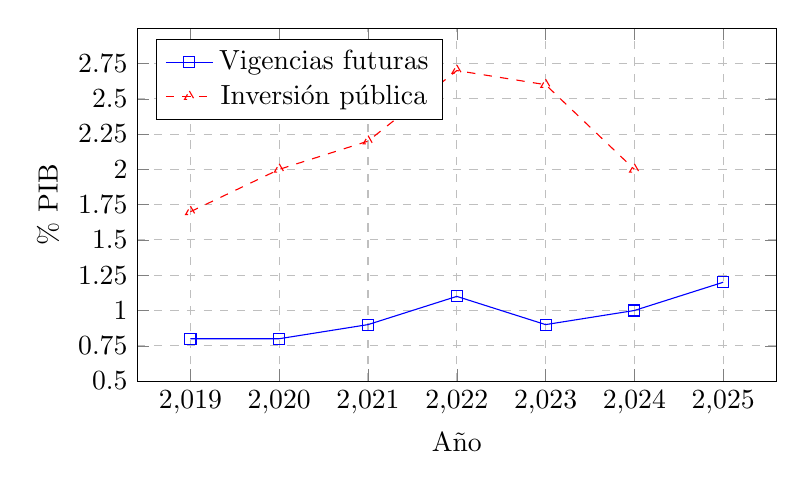
\begin{tikzpicture}
        \begin{axis}[
            width=0.8\textwidth,
            height=0.5\textwidth,
            grid=major,
            xlabel={Año},
            ylabel={\% PIB},
            ymin=0.5, ymax=3.0,
            xtick={2019, 2020, 2021, 2022, 2023, 2024, 2025},
            %ytick={0.5, 1.0, 1.5, 2.0, 2.5},
            ytick={0.50, 0.75, 1.00, 1.25, 1.50, 1.75, 2.00, 2.25, 2.50,2.75},
            legend pos=north west,
            ymajorgrids=true,
            xmajorgrids=true,
            grid style=dashed,
        ]
        \addplot[
            color=blue,
            mark=square,
        ]
        coordinates {
            (2019,0.8)
            (2020,0.8)
            (2021,0.9)
            (2022,1.1)
            (2023,0.9)
            (2024,1.0)
            (2025,1.2)
        };

        \addplot[
            color=red,
            mark=triangle, dashed
        ]
        coordinates {
            (2019,1.7)
            (2020,2.0)
            (2021,2.2)
            (2022,2.7)
            (2023,2.6)
            (2024,2.0)
        };
        \legend{Vigencias futuras, Inversión pública}
        \end{axis}
    \end{tikzpicture}
\vspace{0.3cm}
\par\footnotesize{\textit{Fuente: Elaboración propia con base en Marcos Fiscales de Mediano Plazo 2018--2024 y Balance del GNC, Ministerio de Hacienda.}}
\end{figure}

\begin{comment}
\begin{figure}[h!]
    \caption{Vigencias futuras para inversión (\% PIB)}
    \label{fig:VF}
    \centering
    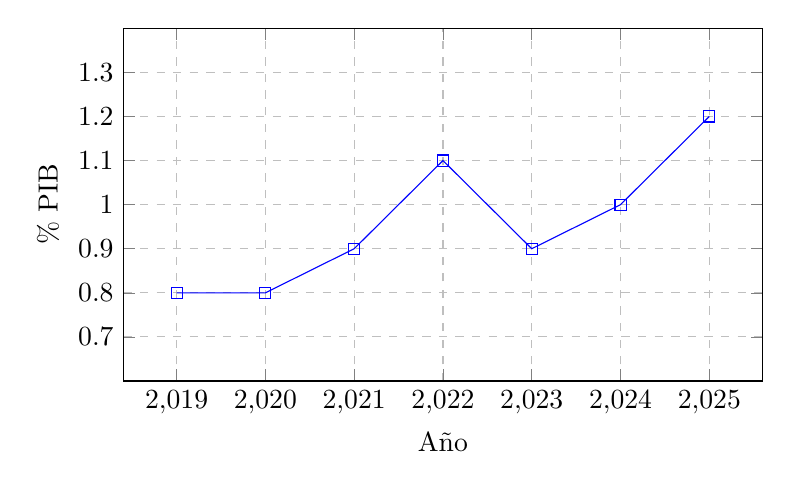
\begin{tikzpicture}
        \begin{axis}[
            width=0.8\textwidth,
            height=0.5\textwidth,
            grid=major,
            xlabel={Año},
            ylabel={\% PIB},
            ymin=0.6, ymax=1.4,
            xtick={2019, 2020, 2021, 2022, 2023,2024,2025},
            ytick={0.7, 0.8, 0.9, 1.0, 1.1, 1.2, 1.3},
            legend pos=north west,
            ymajorgrids=true,
            xmajorgrids=true,
            grid style=dashed,
        ]
        \addplot[
            color=blue,
            mark=square,
            ]
            coordinates {
            (2019,0.8)
            (2020,0.8)
            (2021,0.9)
            (2022,1.1)
            (2023,0.9)
            (2024,1.0)
            (2025,1.2)
            };
        %\legend{VF (\% PIB)}
        \end{axis}
    \end{tikzpicture}
\vspace{0.3cm}
\par\footnotesize{\textit{Fuente: Elaboración propia con base en Marcos Fiscales de Mediano Plazo 2018-2024, Ministerio de Hacienda.}}
\end{figure}
\end{comment}

La Figura \ref{fig:VF} muestra la evolución reciente de las vigencias futuras para inversión y del gasto de inversión pública como porcentaje del PIB. Estas vigencias introducen una rigidez creciente en el gasto público, al pasar del 0,8\% del PIB en 2019 al 1,2\% proyectado para 2025. En contraste, la inversión pública ha venido disminuyendo desde su punto máximo en 2022. La comparación entre ambas series permite dimensionar el peso de las inflexibilidades dentro del gasto de inversión: en 2024, las vigencias futuras representaron cerca de la mitad del total del gasto de inversión. Dado que el presupuesto de inversión —y no el de funcionamiento— constituye el principal instrumento del Gobierno para implementar políticas y programas, estas rigideces reducen significativamente el margen de maniobra de cada administración y limitan su capacidad para redirigir recursos hacia nuevas prioridades.

\section{Gasto de Personal}

Aunque las transferencias y los intereses explican casi la totalidad del aumento del gasto público entre 2019 y 2024, es esencial analizar otros rubros que, si bien no han crecido significativamente, presentan grandes dificultades para ser reducidos. Uno de ellos es el gasto en personal, el cual resulta especialmente complejo de ajustar debido a la autonomía de las entidades gubernamentales, las garantías laborales de los empleados públicos y la importancia de ciertos roles para el funcionamiento del Estado.

El balance fiscal del \gls{gnc} no presenta una desagregación del gasto de personal. No obstante, cada año, el anexo al mensaje presidencial que acompaña el Proyecto de Ley del \gls{pgn} incluye una descomposición de la nómina presupuestada para el año siguiente. Esta nómina puede clasificarse en seis categorías:

\begin{enumerate}[nosep]
  \item La Rama Ejecutiva.
  \item Militares y Policías.
  \item La Rama Judicial, la Rama Legislativa, la Fiscalía y los Organismos de Control.
  \item El personal de educación financiado a través de las transferencias del \gls{sgp} para la educación. 
  \item El personal de salud financiado a través de las transferencias del \gls{sgp} para la salud.
  \item El personal de las universidades públicas.
\end{enumerate}

De estas seis categorías, las últimas tres se financian indirectamente a través de transferencias. Por lo tanto, en términos de contabilidad fiscal del \gls{gnc}, solo las tres primeras se contabilizan como gasto de personal.

\begin{table}[h!]
\centering
\caption{Nómina de la Nación presupuestada para 2025}
\label{tab:Personal}
\begin{tabular}{|>{\arraybackslash}p{9cm}|>{\centering\arraybackslash}p{2cm}|>{\centering\arraybackslash}p{2cm}|}
\hline
\textbf{Sector}                      & \textbf{Cargos (Miles)} & \textbf{Costo (\% PIB)} \\ \hline
1. Rama Ejecutiva & 98 & 0,6 \\ 
2. Militares y Policía & 511 & 1,5 \\ 
3. Judicial, Legislativa y otros  & 88  & 1,0 \\ \hline
\textbf{Financiación x PGN (1+2+3)}  & \textbf{696}  & \textbf{3,1} \\ \hline
4. SGP Educación & 362 & 2,1 \\ 
5. SGP Salud     & 49  & 0,2 \\ 
6. Universidades & 55  & 0,3 \\ \hline
\textbf{Financiación x Transferencias (4+5+6)}    & \textbf{467}  & \textbf{2,6} \\ \hline
\textbf{Gran Total} & \textbf{1163} & \textbf{5,8} \\ \hline
\end{tabular}
\vspace{0.3cm} % Espacio entre la tabla y la fuente
\par\footnotesize{\textit{Fuente: Elaboración propia con base en el Anexo Presidencial del PGN 2025.}}
\end{table}

\begin{comment}
\begin{table}[h!]
\centering
\caption{Nómina 2023 de la Nación}
\label{tab:Personal}
\begin{tabular}{|>{\arraybackslash}p{9cm}|>{\centering\arraybackslash}p{2cm}|>{\centering\arraybackslash}p{2cm}|}
\hline
\textbf{Sector}                      & \textbf{Cargos (Miles)} & \textbf{Costo (\% PIB)} \\ \hline
1. Rama Ejecutiva & 86 & 0,4 \\ 
2. Defensa y Policía & 498 & 1,4 \\ 
3. Judicial, Legislativa y otros  & 80  & 0,8 \\ \hline
\textbf{Financiación x PGN (1+2+3)}  & \textbf{663}  & \textbf{2,6} \\ \hline
4. SGP Educación & 353 & 1,8 \\ 
5. SGP Salud     & 47  & 0,2 \\ 
6. Universidades & 59  & 0,3 \\ \hline
\textbf{Financiación x Transferencias (4+5+6)}    & \textbf{459}  & \textbf{2,3} \\ \hline
\textbf{Gran Total} & \textbf{1122} & \textbf{4,9} \\ \hline
\end{tabular}
\vspace{0.3cm} % Espacio entre la tabla y la fuente
\par\footnotesize{\textit{Fuente: Elaboración propia con base en el Anexo Presidencial del PGN 2023, Ministerio de Hacienda.}}
\end{table}
\end{comment}

La Tabla \ref{tab:Personal} presenta el número de cargos correspondientes a las seis categorías mencionadas y su costo estimado como porcentaje del PIB, con base en la información contenida en el anexo al mensaje presidencial del \gls{pgn}. Para 2025, se presupuestó que la nómina de la Nación ascendería al 5,8\% del PIB. De este total, 2,6 puntos porcentuales corresponden a nóminas financiadas mediante transferencias, mientras que los 3,1 puntos restantes son cubiertos directamente por el \gls{pgn} y se registran como gasto de personal del \gls{gnc}.

De esos 3,1 puntos porcentuales, 1,5 corresponden a Militares y Policías, y 1 punto adicional a la Rama Legislativa, la Rama Judicial, la Fiscalía y los Organismos de Control. En consecuencia, la Rama Ejecutiva representa apenas el 0,6\% del PIB, correspondiente a aproximadamente 98 mil cargos en una Nación con más de 50 millones de habitantes.

Cabe señalar, sin embargo, que el \gls{gnc} también recurre a contratistas bajo la modalidad de prestación de servicios, cuyos costos no se reflejan en el rubro de gasto de personal, sino en el de adquisición de bienes y servicios. Este último se ha mantenido relativamente estable en torno al 0,7\% del PIB entre 2019 y 2024, como se muestra en la Tabla \ref{tab:GastoDesagregado}.

Las nóminas financiadas indirectamente a través de las transferencias operan bajo esquemas que imposibilitan que el \gls{gnc} las reduzca discrecionalmente. Lo mismo ocurre con la nómina de la Rama Judicial, la Rama Legislativa, la Fiscalía y los Organismos de Control. La reducción del número de Militares y Policías sería una iniciativa de una enorme complejidad dados los desafíos de seguridad que enfrenta el país. Aún la posibilidad de ajustar el resto de la nómina de la Rama Ejecutiva enfrenta restricciones legales difíciles de superar dadas las garantías laborales de los empleados públicos. Aún así, la Rama Ejecutiva representa solo el 0,6\% del PIB, lo que hace cuestionar que exista un espacio de recorte sobre el personal de la Rama Ejecutiva lo suficientemente significativo para solventar la situación fiscal. 

Las restricciones asociadas a la reducción de la nómina pública reducen significativamente el margen de maniobra del \gls{gnc} en materia de gasto en personal. Aunque el debate público a menudo se centra en la necesidad de reducir la ``burocracia'', los datos sugieren que cualquier ajuste en este rubro tendría un impacto limitado sobre la sostenibilidad fiscal del país. Dicho esto, el país tiene que estar alerta a los aumentos recientes en el costo de la nómina de la Nación, como se discute en el Capítulo \ref{chap:menosgasto}.

\section{Conclusión}

El aumento del gasto primario entre 2019 y 2024 obedeció casi exclusivamente al aumento de las transferencias. A su vez, las principales transferencias responsables de este aumento fueron el subsidio a los combustibles, la salud y las pensiones. Hacia el futuro, el subsidio a los combustibles tiene una tendencia decreciente, pero otras transferencias como las pensiones, la salud y el \gls{sgp} tiene una tendencia creciente, como se discute en el Capítulo \ref{chap:menosgasto}. Paralelamente, la normalización de un nivel de endeudamiento históricamente alto, amparada por la regla fiscal vigente desde 2022, ocultó la necesidad de reducir la proporción del gasto primario en el PIB a los niveles previos a la pandemia. Este mayor nivel de deuda también provocó un aumento en el pago de intereses como porcentaje del PIB, que, junto con el incremento de las transferencias, explican el crecimiento del gasto total.

\begin{comment}

\input{Tablas/Cap02/rankflex}

Como ejercicio final, vale la pena examinar la composición del gasto público y discutir su grado de flexibilidad. La Tabla \ref{tab:rankflex} clasifica los diferentes rubros del gasto en tres niveles de flexibilidad: altamente inflexible, medianamente inflexible y flexible. Según esta clasificación, las inflexibilidades alcanzaron el 21.6\% del PIB (15.1\% altamente inflexible y 6.5\% medianamente inflexible), mientras que solo el 1.8\% del PIB puede considerarse como gasto público sobre el cual el Gobierno tiene alguna discrecionalidad en el corto plazo.
 
La discusión sobre inflexibilidades deja en el corto plazo los recortes solo pueden aplicarse en rubros como la inversión pública y las transferencias sociales. Sin embargo, reducir estos rubros conlleva grandes desafíos políticos y sociales. En particular, un reducción significativa de la inversión pública dejaría a cualquier gobierno sin posibilidades de recursos para ejecutar un plan de gobierno. A no ser que el principal plan de gobierno sea la consolidación fiscal, como parecería ser la única alternativa de la próxima administración si se quiere frenar la espiral de insostenibilidad de la deuda pública, como se discute en el Capítulo \ref{chap:perspectivas}.

Dado el nivel de inflexibilidades en el presupuesto, cualquier ejercicio de consolidación fiscal se encontrará con restricciones severas. En la práctica, un ajuste súbito del gasto difícilmente podrá superar los 2 puntos del PIB, ya que más allá de ese umbral el recorte implicaría el incumplimiento de compromisos de caracter constitucional o legal. Más aún, una reducción del gasto cercana a 2 puntos del PIB implicaría la paralización de toda inversión pública distinta a la comprometida mediante vigencias futuras. En todo caso, una estrategia de ajuste basada exclusivamente en recortes del gasto es insuficiente y debe complementarse con medidas de incremento de ingresos fiscales, como se argumenta en el Capítulo \ref{chap:perspectivas}.
    
\end{comment}

